
\subsection{Descriptive statistics}

Next, I calculated a number of descriptive statistics for each trial.
Maximum deviation of mouse cursor trajectories was bimodally distributed
(see Chapter 2; Bimodality Coefficient = .567; Hartigan's D = .0224, N = 1499, p < .0001)
and so trajectories were classified as either direct or reversals,
as described in Appendix~\ref{appendix:reversals} (reversal cut-off: MD > 0.972).

When the cues conflicted,
participants who gave the base rate-cued response
spent more time reading the description (3,229 msec, SD = 2,943)
than those who gave the description-cued response
(2,406 msec, SD = 2.789;
$e^{\beta}$ = 125\%, CI = [104\%, 150\%],
t(484.0) = 2.368, p = .018),
and were slower to initiate their mouse movements
(456 msec, SD = 266 vs. 476 msec, SD = 326;
$e^{\beta}$ = 119\%, CI = [110\%, 129\%],
t(486.8) = 4.496, p < .0001),
but did not differ in their response times (p > .5).
Participants were also more likely to
initially move towards the description-cued option
before selecting the base rate-cued one
(38\% of base rate responses)
than to initially move towards the base rate-cued option
and ultimately select the description-cued one
(27\% of description-cued responses;
$e^{\beta}$ = 1.7, CI = [1.03, 2.9],
z = 2.109, p = .035).

\subsubsection{Effect of descriptions on base rate choices}

Table~\ref{tbl:exp5_br_descriptives} shows these descriptive statistics
for trials where the  base rate response was given,
broken down for each type of description.
Table~\ref{tab:exp5_br_betas} shows effect sizes for
the main effect of description type, and pairwise comparisons between descriptions,
for each variable shown in Table~\ref{tbl:exp5_br_descriptives}.

\begin{table}[h]
  \centering
  \caption[Descriptive statistics for base rate-cued responses, Experiment 5.]{
    Descriptive statistics for trials where the base rate-cued response was given in Experiment 5.
    All times are in msec. Standard deviations are shown in parentheses.
    Trials are broken down according to whether the description
    agreed with the base rate, was uninformative,
    or disagreed with the base rate. \\
    \emph{Note:} N = Number of trials in which this response was given.
    \label{tbl:exp5_br_descriptives}
}
  %% \begin{tabular}{lrrrrrrr}
  \begin{tabular}{p{3cm} p{2.5cm} p{2.1cm} p{2.1cm} p{1.75cm} p{1.75cm} }
    \toprule
    %% Condition                  &  \shortstack{Reading time}  & \shortstack{Reading\\time}
    %% & \shortstack{Reading\\time} & Reversals & N   \\
    Description   &  Reading time  & Initiation time & Response time & Reversals & N   \\
    \midrule
    Agreed        &  2,186 (2,153) & 444 (247)       & 1,372 (522)   & 26\%      & 472 \\
    Uninformative &  3,046 (2,890) & 451 (241)       & 1,509 (666)   & 31\%      & 347 \\
    Disagreed     &  3,229 (2,943) & 476 (326)       & 1,776 (739)   & 35\%      & 98  \\
    \bottomrule
  \end{tabular}
\end{table}



There was a significant main effect of
descriptions on reading times
($\chi^2$ = 21.7, N = 2, p < .0001).
When giving the base rate-cued response,
participants were significantly faster to read the description
when it agreed with the base rate (2,186 msec, SD = 2,153)
than when it was uninformative (3,046 msec, SD = 2,890;
$e^{\beta}$ = 76.1\%, CI = [60.9\%, 95.2\%],
t(33.4) = 2.841, p = .0202),
or when it disagreed with it (3,229 msec, SD = 2,943;
$e^{\beta}$ = 70.8\%, CI = [60.1\%, 83.5\%],
t(878.3) = 4.111, p < .0001).
Reading times did not differ between uninformative descriptions
and those that disagreed with the base rate (t < .7, p > .8).

\begin{table}[h]
  \centering
  \caption[Effects of manipulating description on base rate-cued responses, Experiment 5.]{
    Main effects and pairwise comparisons between conditions
    for the effect of condition on the descriptive statistics
    shown in Table~\ref{tbl:exp5_br_descriptives},
    from trials where the base rate-cued response was given.
    For the main effect, the $\chi^2$ statistic is shown,
    which was subjected to a chi-squared test with 2 degrees of freedom in each case.
    For pairwise comparisons, the exponentiated regression weights $e^{\beta}$ are shown,
    reflecting the percentage change in the variables that were log transformed
    (reading, initiation, and response times),
    and the odds ratio change for the binary outcome (reversals).
    \label{tab:exp5_br_betas}
  }
  \begin{tabular}{l L{1.8cm} L{1.8cm} L{1.8cm} l}
    \toprule
    Comparison              & Reading time    & Initiation time & Response time   & Reversals\\
    \midrule
    Main effect ($\chi^2$)  & 21.68 $^{****}$ & 0.42            & 34.93 $^{****}$ & 4.78 $^{.}$\\
    \midrule
    Agreed/Uninformative    & 76\% $^{*}$     &  98\%           & 93\% $^{***}$   & 0.7\\
    Agreed/Disagreed        & 70\% $^{***}$   &  97\%           & 82\% $^{***}$   & 0.7\\
    Uninformative/Disagreed & 93\%            & 99\%            & 89\% $^{**}$    & 0.95\\
    \bottomrule
    \multicolumn{5}{l}{ \emph{Note}: $^{.}$ p < .1; $^{*} p < .05;\ ^{**} p < .01;\ ^{***} p < .001;\ ^{****} p < .0001$ }
  \end{tabular}
\end{table}


Initiation times did not differ according to description type
($\chi^2$ < .5, N = 2, p > .8).
However, there was a main effect of description on response times 
($\chi^2$ = 34.9, N = 2, p < .0001).
Participants were faster to give the base rate-cued response
when the description agreed with the base rate (1,372 msec, SD = 522)
than either when the description was uninformative (1,509 msec, SD = 666)
%% t(29.3) = 3.631, p = .0030),
or when description disagreed with the base rate (1,776 msec, SD = 739).
%% t(980.5) = 5.520, p < .0001)
They were also faster when the description was uninformative
than when it disagreed with the base rate.
%% (t(177.8) = 3.231 , p = 0042).
All comparisons were statistically significant
(t's > 3.2, p's < .01).

There was a marginally significant effect of descriptions on reversals
---  the probability of initially moving towards
the alternative option before giving the base rate response
($\chi^2$ = 4.8, N = 2, p = .0916).
Despite this, none of the post-hoc comparisons approached significance.
However, the trends were in the direction predicted by dual process accounts.
On trials where participants gave the base rate-cued response,
a greater proportion changed their mind while doing so
when the description cued the opposite response
than when the description was uninformative,
and fewer again did so when the description agreed with the base rate.

In summary, consistent with what would be predicted by most dual process accounts,
participants were indeed slower to give the base rate-cued response
when it went against the contents of the description,
and spent longer reading the description for such problems.
For trials where the base rate-cued response was given,
descriptions did not have a significant effect
on participants' initial cursor movements, in contrast to previous experiments.
This pattern, however, can be better understood
by considering the transition probability analyses, below.


\subsubsection{Effect of base rates on description choices}

Table~\ref{tab:exp5_d.descriptives} shows descriptive statistics
for trials in which the description-cued response was given, by condition.
Contrary to a number of previous studies that found evidence that
base rates interfere with participants' description-cued responses,
there was no main effect of condition found on any of the descriptive measures here
($\chi^2$  < 3.4, DF = 2, p > .18).
Focusing on response time, the measure most commonly analysed in previous studies,
reveals a weak trend in the expected direction.
Response times when both cues agreed (1,372 msec, SD = 522)
were almost identical to when only the description was informative (1,369 msec, SD = 464),
but slightly faster than when the base rate cued the opposite response (1,402 msec, SD = 563).

\begin{table}[h]
  \centering
  \caption[Descriptive statistics for description-cued responses, Experiment 5.]{
    Descriptive statistics for trials where the description-cued response
    was given in Experiment 5.
    Trials are broken according to whether the base rate
    agreed with the description, was uninformative,
    or disagreed with the description.\\
    \emph{Note:} N = Number of trials in which this response was given.
    \label{tab:exp5_d.descriptives}
  }
  %% \begin{tabular}{lrrrrrr}
  \begin{tabular}{p{3cm} p{2.5cm} p{2.1cm} p{2.1cm} p{1.75cm} p{1.75cm} }
    %% Condition        & \shortstack{Description\\Responses} & 
    %%                    \shortstack{Reading\\time} &
    %%                    \shortstack{Initiation\\time} & 
    %%                    \shortstack{Response\\time}  &
    %%                    Reversals & N  \\
    %% Condition        & Reading time  & Initiation time & Response time & Reversals & N  \\
    %% Condition                  &  \shortstack{Reading time}  & \shortstack{Reading\\time}
    %% & \shortstack{Reading\\time} & Reversals & N   \\
    \toprule
    Base rate     &  Reading time & Initiation time & Response time & Reversals & N   \\
    \midrule
    Agreed        & 2,186 (2,153) & 444 (247)       & 1,372 (522)   & 29\%      & 472\\
    Uninformative & 2,309 (2,260) & 447 (258)       & 1,369 (464)   & 28\%      & 467\\
    Disagreed     & 2,406 (2,789) & 456 (266)       & 1,402 (563)   & 27\%      & 401\\
    \bottomrule
  \end{tabular}
\end{table}


In previous tests of the intuitive logic theory
\citep[e.g.][see also \citealp{Pennycook2015}]{DeNeys2011b,Mevel2014},
researchers have explored the relationship between
individual differences in overt sensitivity to normative principles
(i.e. the proportion of normatively correct responses given on conflict trials)
and implicit measures of  conflict.
Therefore, I calculated, for each participant,
the proportion of description-cued responses on conflict trials.
Of the 50 participants, 26 gave the description-cued response
on 9 or 10 of the 10 conflict trials,
and were classed as \emph{description-driven reasoners}.
The remaining 24 participants gave
the description-cued response on average 62\% of the time,
and were classed as \emph{equivocal reasoners}.
Only 4 of these participants gave the base rate-cued response
on more than half of the conflict trials.

I repeated the analyses described above ---
analysing reading time, movement initiation time, response time, and proportion of reversals,
on trials where the base rate-cued response was given ---
using 3 (description: agreed, uninformative, or disagreed with base rate)
by 2 (type of reasoner: description-driven or equivocal) factorial mixed models,
with random intercepts for each participant and each problem.
None of these models showed significant description by type of reasoner interactions (p's > .1),
indicating that there were no substantial individual differences in
the null effects of manipulating the description reported above.


However, the analyses reported here are in some ways conservative.
Working within the null hypothesis significance testing (NHST) framework,
I have calculated p values, comparing the main effect of base rate types
on participants' response times to what would be expected under the null hypothesis.
Because there were three kinds of base rate ---
they could agree with the descriptions, be uninformative, or disagree ---
I then performed pairwise comparisons,
using the Tukey HSD method to adjust the p values
to maintain a Type 1 error rate of 5\%.
While I was unable to reject the null hypothesis
--- that base rates did not influence participants
on trials where they gave the description-cued response ---
this framework does not make it possible to accept this null hypothesis either.

Therefore, I conducted a follow up analysis,
comparing responses where the base rate agreed with the description
to those where it disagreed,
and used Bayesian inference to estimate
the magnitude of the difference in response time between these two conditions.
Participants on average responded in 1,372 msec (SD 522 msec) when the cues agreed,
and 1,402 msec (SD 563 msec) when they disagreed, a slowdown of 30 msec, or 2.1\%.

I fit a Bayesian multilevel model using Stan 
\citep{StanDevelopmentTeam2015},
where log-transformed response times for
description-cued responses when the base rate agreed with the description
where compared to those where the base rate disagreed.
The model included random intercepts
for each participant, and for each problem.
Uninformative priors were set on all model parameters.
The full model specification can be found in Appendix~\ref{appendix:exp5_bayes}.

After sampling,%
\footnote{
  I ran 8 MCMC chains of 1000 iterations each,
  with 500 warm-up draws discarded from each chain.
  }
the posterior distribution for the intercept term
(the mean response time when the base rate agreed),
had a median estimate of 1,357 msec
and a 95\% credible interval%
\footnote{
  A Bayesian 95\% credible interval can be interpreted in the way
  that frequentist confidence intervals are often misinterpreted:
  we can be 95\% sure that the true value
  lies between these lower and upper bounds,
  given our prior beliefs and the current data.}
of [1,285 msec; 1,423 msec].
More importantly, posterior on the regression weight $e^{\Beta}$
is shown in Figure~\ref{fig:exp5_posterior}.
The median estimate was 102.8\%, indicating a 2.8\% slowdown under conflict,
and the 95\% credible interval was [99.0\%; 106.7\%].
Therefore, while the most credible effect is a very small slowdown under conflict,
there is considerable uncertainty around this effect.
We can further understand this estimate by looking to
the mass of the posterior above and below certain values.
For instance, we can be 91.9\% certain
that response times under conflict were \emph{slower} than those when the cues agreed
--- that is, $e^{\beta}$ > 100\% ---
but also 99.1\% certain that the slowdown did not exceed 10\%
of the response time when the cues agreed.
Another way of interpreting a posterior of this sort \citep{Kruschke2011}
is to define a range of effect sizes that we would consider to be trivial
--- that is, to define a \emph{region of practical equivalence}; ROPE.
For us to be 95\% confident that this effect constitutes a null result,
we would need to define all changes in response time
from 94\% to 106\% as being essentially null effects.
As I believe that effects within this range would be of theoretical importance,
the current results do not support the null hypothesis.



\begin{figure}[ht]
  \centering
  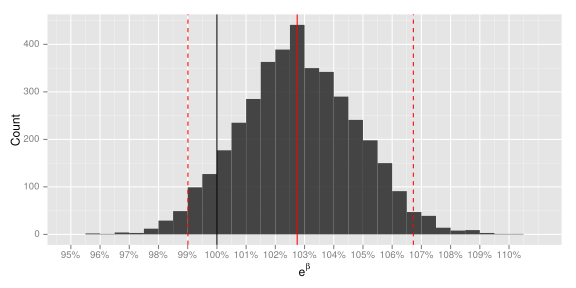
\includegraphics[width=.75\textwidth]{imgs/posterior.pdf}
  \caption[Bayesian analysis of effect of the base rate
    on rt for description-based responses, Experiment 5.]{
    \label{fig:exp5_posterior}
    Posterior samples for the $e^{\beta}$ regression weight,
    reflecting the difference in response times
    between description-based responses when the base rate agreed with the description
    and those when the base rate disagreed.
    The median estimate of 102.8\%
    (solid red line, dashed lines show 95\% credible intervals)
    indicates that participants were 2.8\% slower when the base rate disagreed.
    The solid black line shows the null effect.
  }
\end{figure}

In summary, the evidence here was not sufficient
to reject the null hypothesis in a NHST ANOVA design.
However, when I directly contrasted trials where
the base rate agreed with the description
to those where they disagreed,
the data supported an extremely small conflict effect with considerable uncertainty,
rather than the null hypothesis of no effect whatsoever.
Ultimately, the present data are inconclusive,
and fail to provide strong evidence
either of a slow-down under conflict,
or of the absence of such a slow-down.
